\chapter{Experimentation}
\label{experimentation}
The goal of this chapter is to evaluate our adaptive SPS, both the reactive and predictive approaches. In this way, we will analyze the impact of adaptation on the performance of the SPS. %For comparison, there will be three sections: adaptive SPS, \rSPS{} and \pSPS{}.

Section \ref{exp:scenario} presents the experimental scenario, specifying the environment, the dataset, the parameters and the evaluation metrics. Section \ref{exp:modified-sps} presents the evaluation of our extended version our extended version of Storm, which uses a replica pool and \textit{Load-aware} grouping. Section \ref{exp:reactive} presents the evaluation and analysis of \rSPS{}, using different configurations in their weights and applications. Finally, Section \ref{exp:predictive} presents the evaluation and analysis of \pSPS{}, both of the parametrization used as well as a comparison with other existing adaptive SPS.

\section{Experiment scenario}
\label{exp:scenario}
In this section, we describe the components necessary for the creation of an experiment scenario, which has three components: environment, dataset and application. For each experiment, we considered a set of measures for which the difference in behaviour was negligible.

Section \ref{exp:enviroment} presents the environment that is the architecture used for the deployment of the adaptive SPS. Section \ref{exp:dataset} presents the dataset refers to the traffic used to provide an input data stream. Section \ref{exp:app} presents the applications designed with its respective processing according to the DAG and the type of data used. Section \ref{exp:params} presents the parameters used by the adaptive SPSs. Finally, Section \ref{exp:metric} presents the evaluation metrics.
 
\subsection{Environment} 
\label{exp:enviroment}
All the experiments were conducted on the Google Cloud Platform (GCP) using seven Virtual Machines (VMs): three in charge of Zookeeper, seven as Supervisor nodes, and one for running both the Nimbus and the adaptive SPS. Our test environment is presented in Figure \ref{fig:exp-testbed}. 

Three types of machines were used: a \texttt{n1-standard-1} (1 CPU, 2.2 GHz, 3.75 GB of RAM) machine for hosting Zookeeper VMs, a \texttt{n1-standard-4} (4 CPU, 2.2 GHz, 15 GB of RAM) for Nimbus and the adaptive SPS, and a \texttt{n1-highcpu-8} (8 CPU, 2.2GHz, 7.2GB of RAM) machine for the Supervisors VMs.

\begin{figure}[!ht]
      \centering
     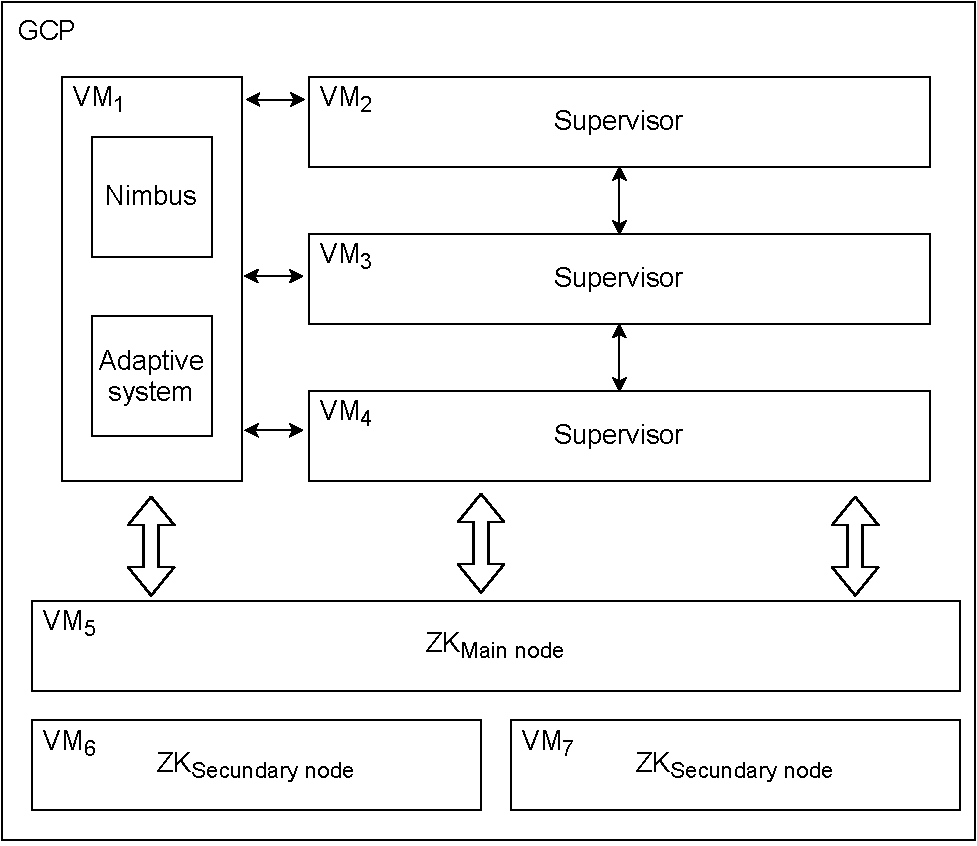
\includegraphics[width=0.65\textwidth]{figures/exp/GCP.pdf}
     \caption{Development environment on GCP.}
     \label{fig:exp-testbed}
\end{figure} 
 
\subsection{Dataset}
\label{exp:dataset}
We have considered four dataset for the experiments: \textit{Twitter Gaussian}, \textit{Twitter Smoothed}, \textit{Twitter Raw}, \textit{Logs} and \textit{DNS}.

\begin{itemize}
\item \textit{Twitter Gaussian}: This dataset is traffic that follows a Gaussian distribution, whose data are tweets related to COVID-19 \cite{PXF2CU2020}. Figure \ref{fig:exp-dataset-twitter-gaussian} shows the traffic provided by this distribution.

\begin{figure}[!ht]
\centering
    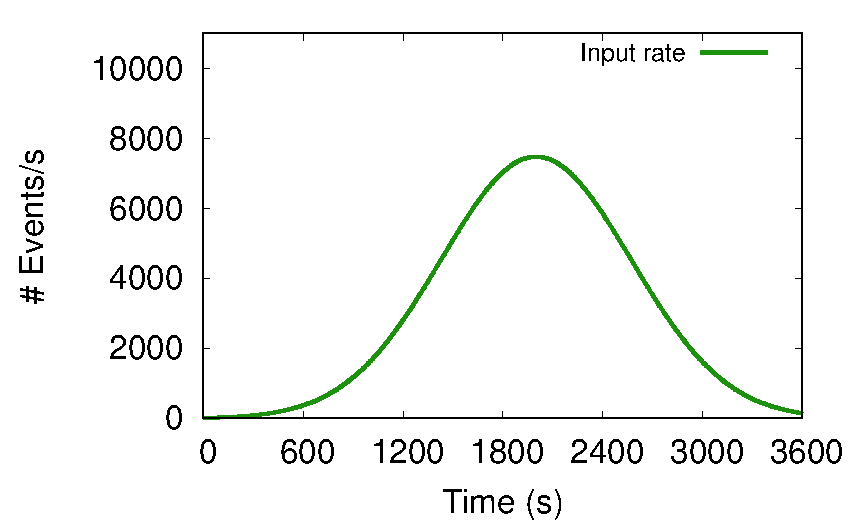
\includegraphics[width=0.5\textwidth]{figures/exp/Dataset-TwitterGaussian.pdf}
    \caption{Traffic shape of Twitter Gaussian dataset.}
    \label{fig:exp-dataset-twitter-gaussian}
\end{figure}

\item \textit{Twitter Raw}: This dataset is based on data from Twitter related to COVID-19, with 237 million tweets \cite{PXF2CU2020}. Figure \ref{fig:exp-dataset-twitter-raw} shows the traffic provided by this dataset.

\begin{figure}[!ht]
\centering
    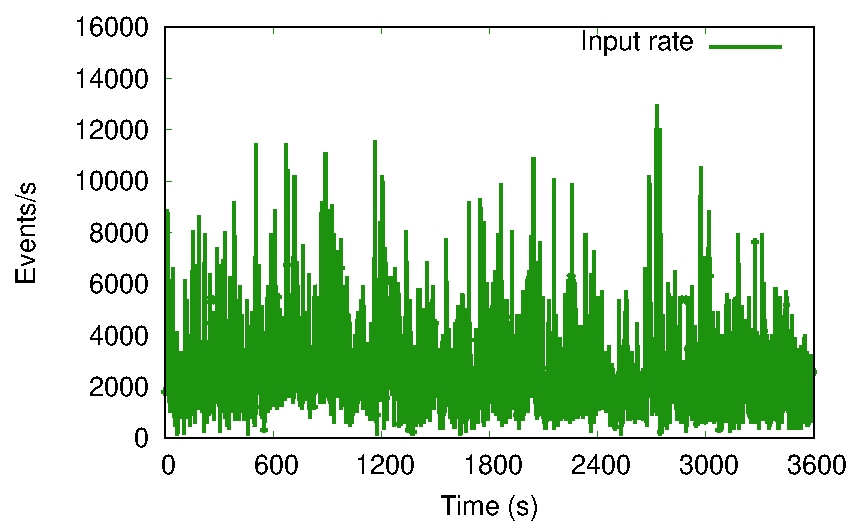
\includegraphics[width=0.5\textwidth]{figures/exp/Dataset-TwitterRaw.pdf}
    \caption{Traffic shape of Twitter Raw dataset.}
    \label{fig:exp-dataset-twitter-raw}
\end{figure}

\item \textit{Twitter Smoothed}: This dataset is based on \textit{Twitter Raw}. However, we have considered only a sample of these tweets in the experiments, i.e., those in periods of the datasets that present high rate variation. In other words, we select a combination of traffic spikes and under spikes to compose the input traffic for the experiments. The methodology adopted to build the testing dataset was introduced in \cite{BodikFFJP10}. Figure \ref{fig:exp-dataset-twitter-raw} represented the traffic designed \ref{fig:exp-dataset-twitter-smoothed}.

\begin{figure}[!ht]
\centering
    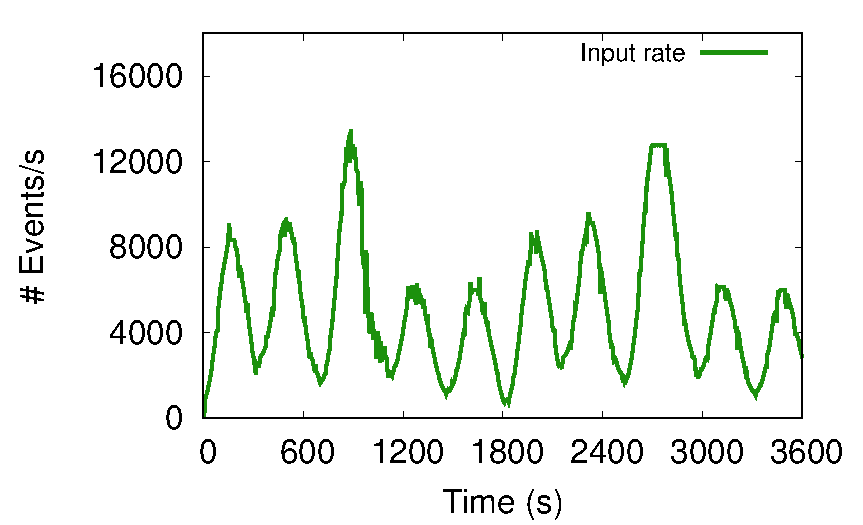
\includegraphics[width=0.5\textwidth]{figures/exp/Dataset-TwitterSmoothed.pdf}
    \caption{Traffic shape of Twitter Smoothed dataset.}
    \label{fig:exp-dataset-twitter-smoothed}
\end{figure}

\end{itemize}

\begin{itemize}
\item \textit{DNS}:  This dataset is based on network traffic, which was created to test DNS over HTTPS, a more secure version of the DNS protocol \citep{MontazeriShatoori20}. We used the same methodology mentioned above was used to build the dataset. Figure \ref{fig:exp-dataset-dns} shows the log traffic provided by this dataset.
\end{itemize}

\begin{figure}[!ht]
\centering
    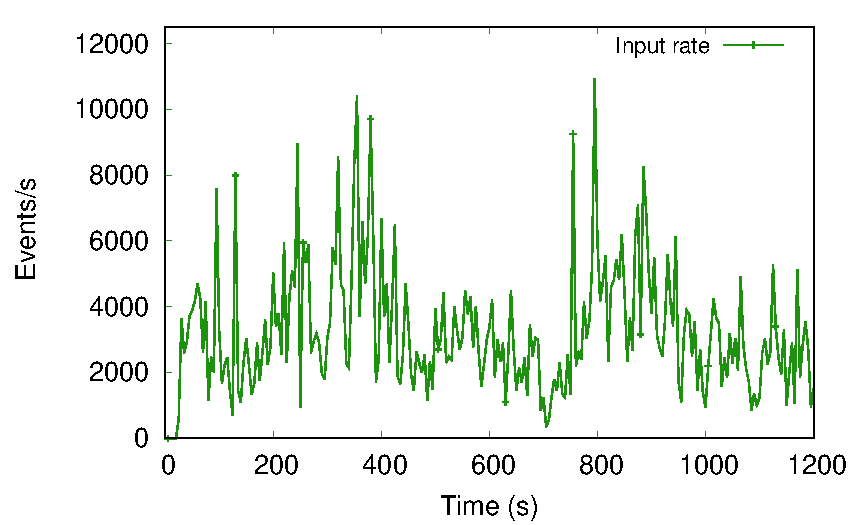
\includegraphics[width=0.5\textwidth]{figures/exp/Dataset-DNS.pdf}
    \caption{Traffic shape of DNS dataset.}
    \label{fig:exp-dataset-dns}
\end{figure}

\begin{itemize}
\item \textit{Log}: This dataset is based on system logs from a distributed system  \citep{LogsPaper}. We used the same methodology mentioned above was used to build the dataset. Figure \ref{fig:exp-dataset-log} shows the log traffic provided by this dataset.
\end{itemize}

\begin{figure}[!ht]
\centering
    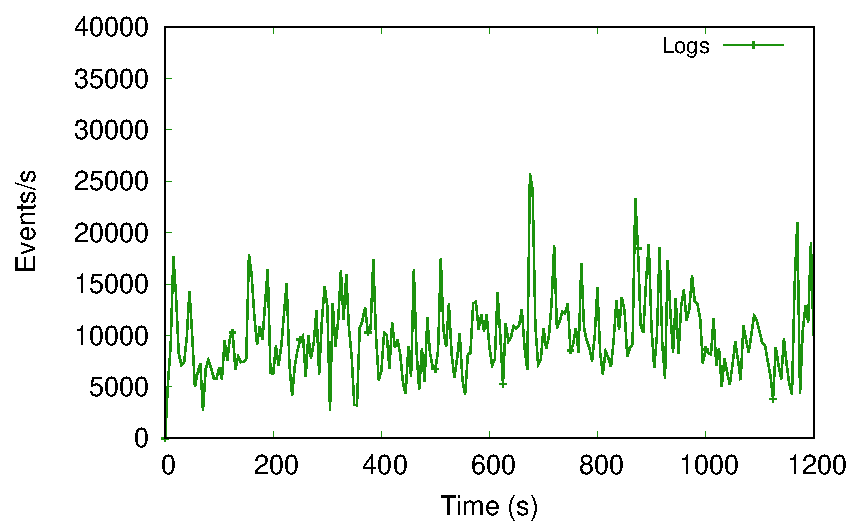
\includegraphics[width=0.5\textwidth]{figures/exp/Dataset-Logs.pdf}
    \caption{Traffic shape of Log system dataset.}
    \label{fig:exp-dataset-log}
\end{figure}

\subsection{Application}
\label{exp:app}
For each traffic, we have at least one application to be used. The applications designed for the experimental phase are listed below:

\begin{itemize}
\item \textit{Twitter linear}: It is a linear DAG for \textit{Twitter} dataset, which is composed of four operators.

\begin{itemize}
	\item \textit{Detection}: Its goal is to detect tweet events of a Twitter data streaming according to a topic, subtopic, category, and subcategory list of keywords. Each operator has one of these lists and verifies if any of the words of a tweet is included in the list in question. Therefore, in the sequence, the first, second, third, and fourth operators respectively determine the topic, subtopic, category, and subcategory of each tweet as shown in Figure \ref{fig:app-twitter-linear-1}.
	
\begin{figure}[!ht]
\centering
    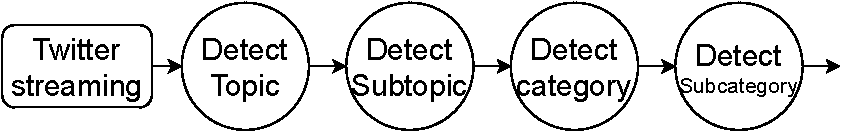
\includegraphics[width=0.65\textwidth]{figures/exp/App-Twitter-Linear-1.pdf}
    \caption{Detection Twitter application in SPS.}
    \label{fig:app-twitter-linear-1}
\end{figure}	
	
	\item \textit{Classification}: Its goal is to classify tweet events of a Twitter data streaming. The first classifier determines whether the text is positive, negative or neutral, and the second identifies the person who has published them. Classified tweets are stored in a database. Figure \ref{fig:app-twitter-linear-2} shows this application.
\begin{figure}[!ht]
\centering
    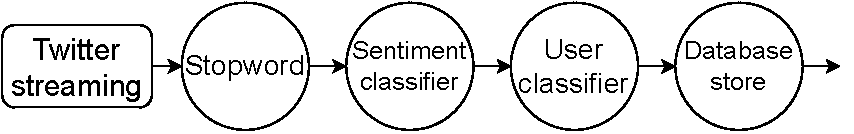
\includegraphics[width=0.65\textwidth]{figures/exp/App-Twitter-Linear-2.pdf}
    \caption{Classification Twitter application in SPS.}
    \label{fig:app-twitter-linear-2}
\end{figure}			
\end{itemize}

\item \textit{Twitter complex}: It is a complex DAG for \textit{Twitter} dataset, which is composed of eight operators. Figure \ref{fig:app-twitter-complex} shows the DAG of this application. It analyses Twitter streaming containing information such as news or opinions. Depending on the type of information, the stream can be split. Finally, results are stored in a database.

\begin{figure}[!ht]
\centering
    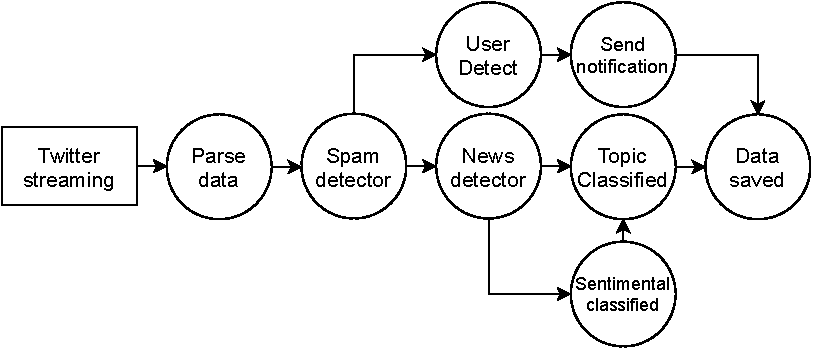
\includegraphics[width=0.75\textwidth]{figures/exp/App-Twitter-Complex.pdf}
    \caption{Classification Twitter application in SPS.}
    \label{fig:app-twitter-complex}
\end{figure}

\item \textit{Log}: It is a linear DAG for \textit{Log} dataset, which is composed of four operators. Figure \ref{fig:app-log} shows its representation of DAG. Its objective is to determine the importance of the log trace.

\begin{figure}[!ht]
\centering
    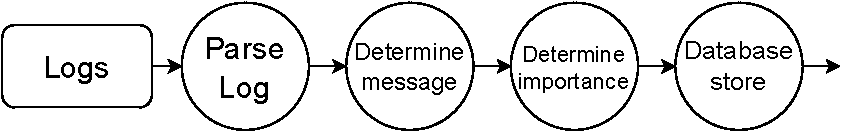
\includegraphics[width=0.65\textwidth]{figures/exp/App-Log.pdf}
    \caption{Log application in SPS.}
    \label{fig:app-log}
\end{figure}

\item \textit{DNS}: It is a linear DAG for \textit{DNS} dataset, which is composed of four operators. Figure \ref{fig:app-dns} shows its representation of DAG. Its goal is analyses and classifies events based on DNS traffic.

\begin{figure}[!ht]
\centering
    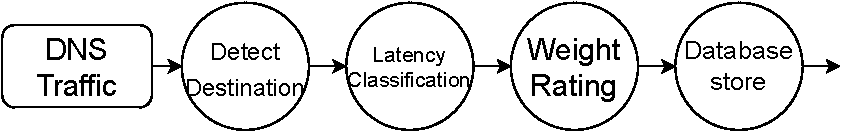
\includegraphics[width=0.65\textwidth]{figures/exp/App-DNS.pdf}
    \caption{DNS application in SPS.}
    \label{fig:app-dns}
\end{figure}

\end{itemize}

\subsection{Parameters}
\label{exp:params}
Table \ref{tab:exp-reactive-parameters} summarizes \rSPS{} parameters and their respective values. These values were determined according to expertise and learning outcomes obtained from the results of several previous experiments using different parametrizations.

\begin{table}[!ht]
\centering
\begin{tabular}{|c|l|c|}
\hline
Parameter     & Description & Value
\\ \hline \hline
$td$          & Time interval duration & 25 sec  \\ \hline
$\delta_{u}$    & Operator state upper limit & 0.7     \\ \hline
$\delta_{l}$    & Operator state lower limit   & 0.3     \\ \hline
$\delta_{E}$    & Limit for adding replicas  & 0.7     \\ \hline
$\omega_U$    &  $U$ metric weight & 0.45    \\ \hline
$\omega_Q$    & $Q$ metric weight & 0.45    \\ \hline
$\omega_E$    & $E$ metric weight & 0.1     \\ \hline
$k$  		  & Number of active replicas to add/remove & 1       \\ \hline
\end{tabular}
\caption{\rSPS{} parameters and their values.}
\label{tab:exp-reactive-parameters}
\end{table}

Table \ref{tab:exp-predictive-parameters} summarizes \pSPS{} parameters and their respective values. To determine the values of predictive model parameters, the model has considered obtaining a representative sampling based on the methodology presented in \citep{winters2017practical}.

\begin{table}[!ht]
\centering
\begin{tabular}{|c|l|c|}
\hline
Parameter     & Description & Value
\\ \hline \hline
$td$   & Time interval duration    							    & 30 sec  \\ \hline
$to$   & Observation time interval duration for predictor model & 1 sec    \\ \hline
$s$    & Number samples for predictor model     				& 100  \\ \hline
\end{tabular}
\caption{\pSPS{} parameters and their values.}
\label{tab:exp-predictive-parameters}
\end{table}

For \textit{Storm} parameters, we used default values \footnote{http://github.com/apache/storm/blob/master/conf/defaults.yaml}, except timeout to detect the failure of an event, $t_{out}=30s$, and queue size, $q_{size}=100000$. 

\subsection{Metrics}
\label{exp:metric}
For the evaluation, we have defined six evaluation metrics.
\begin{itemize}
    \item \textit{Saved resources}: proposed in \cite{LombardiABQ18}, this metric expresses the proportion of resources (active replicas) saved with respect to a statically over-provisioned configuration.
    It is defined by  $1-\frac{r}{r_{over}}$, with $r$ the number of active replicas, and $r_{over}$ the overestimated number of replicas. $r_{over}$ is the number of replicas needed to process all the events during the highest input rate peak of the benchmark. Note that if the value of the metric is close to 1, a high number of resources has been saved.
    \item \textit{Throughput degradation}: this  metric, also described in \cite{LombardiABQ18}, aims at analyzing the behavior of the system in terms of throughput stability. It is defined by  $\frac{\left | input_{rate} - output_{rate} \right |}{input_{rate}}$.  If the metric value is close to 0, the system has a good stability. On the other hand, if it is close to 1, the system is not capable to process the input rate and the system is unstable.
    \item \textit{Latency}: is the average time taken by an event between the moment it enters and leaves the SPS (end-to-end latency). This metric is relevant since SPSs are supposed to deliver real-time processed events.
    \item \textit{Difference in the number of processed events}: is the difference between the total number of processed events and the total number of received events. It is an important metric since SPSs are used to process high volumes of data.
    \item \textit{Error estimation input}: is the mean absolute percentage error of the difference between the input rate and the predicted input rate during each interval.
    \item \textit{Error estimation replica}: is the mean absolute percentage error of the difference between the number of replicas needed to process all events and the number of predicted replicas during each interval.
\end{itemize}

\section{Impact of the new features}
\label{exp:modified-sps}

The aim of this section is to evaluate the modifications made to our SPS, being an extension of \textit{Storm}, with respect to the standard version of \textit{Storm}. These modifications are described in Section \ref{modified-sps}, which correspond to \textit{Pool of replica} (Section \ref{exp:pool}) and \textit{Load-Aware} grouping (Section \ref{exp:grouping}). 
%% NOTE !!!!
%It is important to note that different approaches were used in the experiments, as the evaluations were carried out in different publications.


\subsection{Pool of replica}
\label{exp:pool}
In this experiment, we compared Storm, denoted  \textit{Storm-Default}, with our modified version of Storm that uses the pool of replicas, denoted \textit{Storm-Pool}, described in Section \ref{pool}. We used the \textit{Twitter Gaussian} dataset, the \textit{Twitter linear - Detection} application, \textit{Shuffle grouping} for stream grouping strategy. Both versions of Storm use the \textit{reactive approach} presented in Section \ref{reactive-approach}. Note that Gaussian traffic shape allows to evaluate the capacity of the system to scale-out and scale-in. For calculating the \textit{Saved resources} metric, we have fixed $r_{over} = 60$ (i.e., $r_i = 15$). The size of each pool of replicas ($p$) was set to 12. Table \ref{tab:exp-pool} summarizes the results obtained for each metric.

\begin{table}[!ht]
\centering
\begin{tabular}{|l|llll|}
\hline
System & \begin{tabular}[c]{@{}l@{}}Saved\\ Nodes\end{tabular} & \begin{tabular}[c]{@{}l@{}}Throughput\\ Degradation\end{tabular} & \begin{tabular}[c]{@{}l@{}}Diff. Processed\\ Events\end{tabular} & \begin{tabular}[c]{@{}l@{}}Latency\\ (ms)\end{tabular} \\ \hline \hline
Storm-Pool      & 0.2038   & 0.2039 & 0.9987 & 12121.92 \\ \hline
Storm-Default   & 0.2041   & 0.4031 & 0.8627 & 913.10 \\ \hline
\end{tabular}
\caption{System metric values of \textit{Storm-Pool} and \textit{Storm-Default} using \textit{Twitter Gaussain} dataset.}
\label{tab:exp-pool}
\end{table}

Figure \ref{fig:exp-pool-replicas} presents the number of replicas required by each of the two systems. We observe that the difference between both curves is not very significant. Furthermore, the difference in \textit{Saved nodes}  values of both systems shown in  Table \ref{tab:exp-pool} is of $0.03\%$ and, in terms of  memory usage, \textit{Storm-Pool} requires only $2.6\%$ of extra memory when compared to \textit{Storm-Default}, which is due to the pre-allocation of the pools of replicas when deploying the application.

\begin{figure}[!ht]
    \centering
    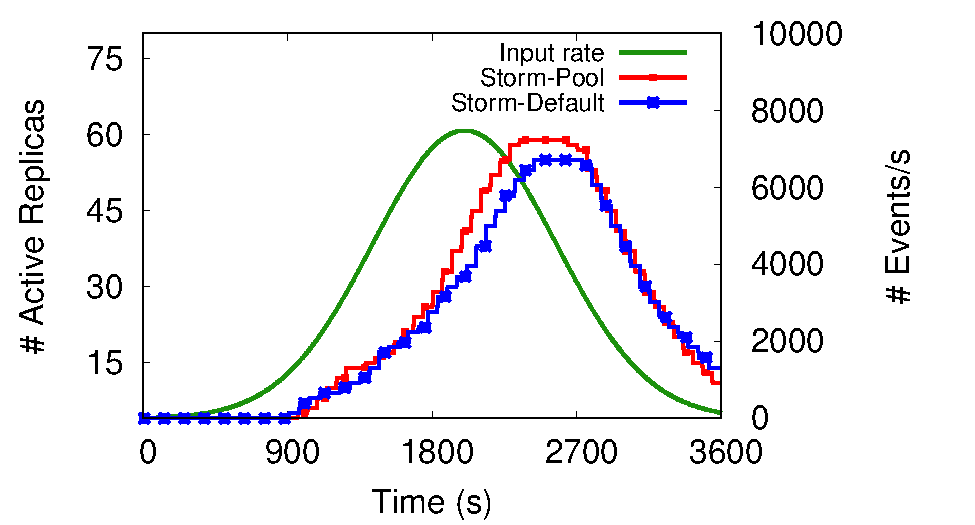
\includegraphics[width=0.75\textwidth]{figures/exp/storm/Pool-Replicas.pdf}
    \caption{Total number of replicas of \textit{Storm-Pool} and \textit{Storm-Default}.}
    \label{fig:exp-pool-replicas}
\end{figure}

Figure \ref{fig:exp-pool-throughput} shows the output data rate for each system. The main drawback of \textit{Storm-Default} is the need to restart the system at each reconfiguration. We can observe that output rates drop at each reconfiguration.
On the other hand, \textit{Storm-Pool} exploits the preloaded replicas that enable the system to process events continuously while adapting itself. Table \ref{tab:exp-pool} shows a difference of almost $20\%$ on \textit{throughput degradation} between both systems.

\begin{figure}[!ht]
    \centering
    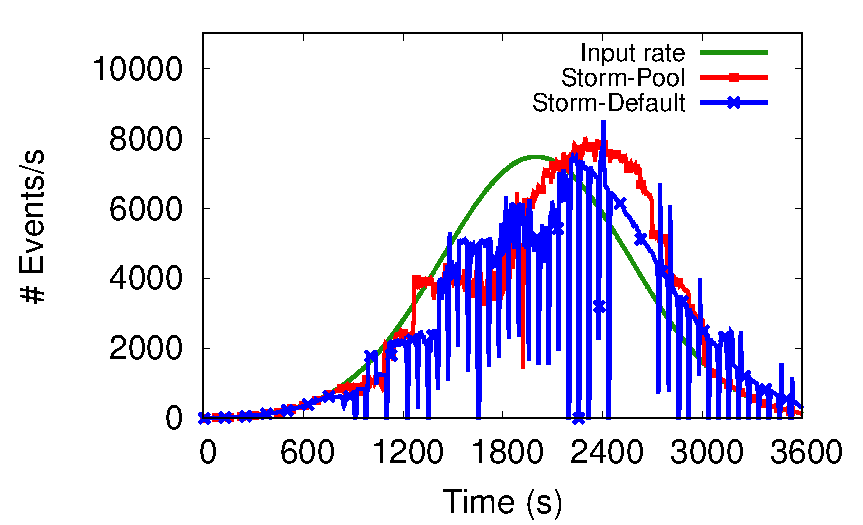
\includegraphics[width=0.75\textwidth]{figures/exp/storm/Pool-Throughput.pdf}
    \caption{Throughput of \textit{Storm-Pool} and \textit{Storm-Default}.}
    \label{fig:exp-pool-throughput}
\end{figure}

The number of cumulative processed events is shown in Figure \ref{fig:exp-pool-exec-total}. Once again, we can observe the impact of reconfiguration downtime over the performance of the \textit{Storm-Default}: there is a $13.6\%$ difference between both systems in terms of the total number of processed events. We highlight  that message loss in real stream processing applications can be critical (e.g., fraud detection systems). 

Therefore, based on the above results and discussions, we can conclude that Storm reconfiguration approach is not suitable for real-time applications that require timely responses. 

\begin{figure}[!ht]
    \centering
    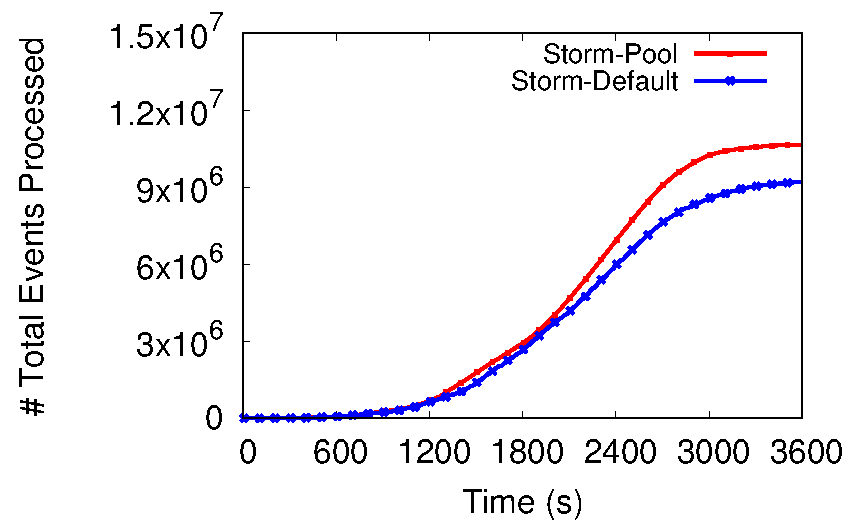
\includegraphics[width=0.75\textwidth]{figures/exp/storm/Pool-ExecutedTotal.pdf}
    \caption{Total number of processed events of \textit{Storm-Pool} and \textit{Storm-Default}.}
    \label{fig:exp-pool-exec-total}
\end{figure}

Figure \ref{fig:exp-pool-latency} evaluates the latency for both implementations. The difference in latency is $92.46\%$  between the two systems. The availability of the system explains this huge difference. On the one hand, \textit {Storm-Pool} is always available to process incoming data. On the other hand, \textit {Storm-Default} is down during the reconfiguration phase. 
In this way, there is a greater number of queued events part of the \textit {Storm-Pool}, resulting in an increase in latency.

\begin{figure}[!ht]
     \centering
     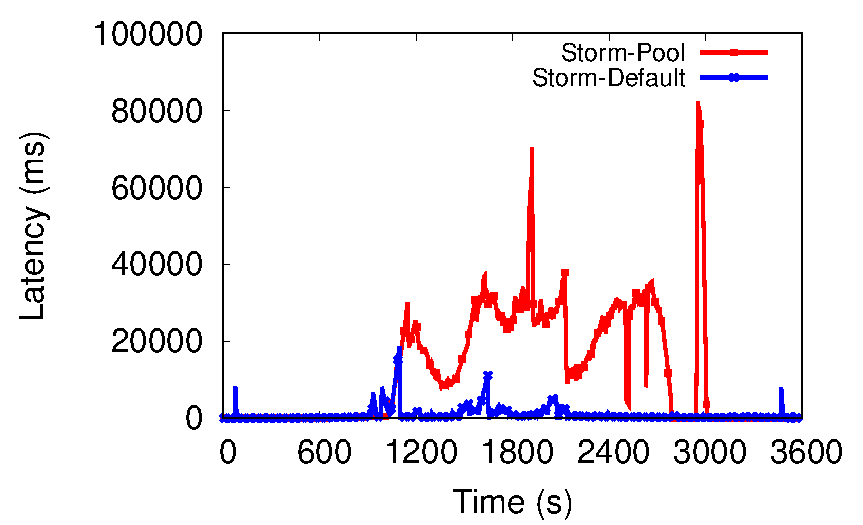
\includegraphics[width=0.75\textwidth]{figures/exp/storm/Pool-Latency.pdf}
     \caption{Comparison of latency between \textit{Storm-Default} and \textit{Storm-Pool}.}
     \label{fig:exp-pool-latency}
 \end{figure}

We should also point out that the MAPE integrated in our SPS does not use much more extra resources since the monitored information exploited by it is the same one collected by Nimbus. Furthermore, MAPE algorithms do not require much computation time because they just consist in simple mathematical calculations according to the formulas presented.

\subsection{Grouping}
\label{exp:grouping}
This experiment compares our stream grouping strategy, denoted \textit{Load-Aware Grouping}, described in Section \ref{grouping} with the shuffle grouping where events are randomly distributed among the replicas. We used the \textit{Twitter Smoothed} dataset, the \textit{Twitter linear - Classification} application and the \textit{predictive approach} (\pSPS{})\footnote{Load-Aware grouping has only been implemented in \pSPS{}, so \rSPS{} cannot use it.}, which used \textit{Basic} model for input prediction. For calculating the \textit{Saved resources} metric, we have fixed $r_{over} = 32$ (i.e., $r_i = 8$). The size of each pool of replicas ($p$) was set to 12.

Table \ref{tab:exp-grouping} shows the metrics for both grouping strategies. There is no significant difference in terms of processed events  and only an increase of $4.04\%$ in saved resources using our grouping strategy. Regarding the use of VMs resources, CPU utilization increases by $0.9\%$ with respect to a random distribution and the difference in memory usage is negligible.

\begin{table}[!ht]
\centering 
\begin{tabular}{|l|llll|}
\hline Grouping
& \begin{tabular}[c]{@{}l@{}}Saved\\ Resources\end{tabular} & \begin{tabular}[c]{@{}l@{}}Throughput\\ Degradation\end{tabular} & \begin{tabular}[c]{@{}l@{}}Diff. Proc.\\ Events\end{tabular} & \begin{tabular}[c]{@{}l@{}}Latency\\ (ms)\end{tabular} \\ \hline \hline
Shuffle             & 0.5390   & 0.4332 & 0.9979 & 5271.01 \\ \hline
Load-Aware      & 0.5617   & 0.1831 & 0.9987 & 2098.91 \\ \hline
\end{tabular}
\caption{System metric values of \textit{Load-Aware} and \textit{Shuffle} grouping using \textit{Twitter Gaussain} dataset.}

\label{tab:exp-grouping}
\end{table}

On the other hand, there is a great difference in latency and throughput metrics of the two strategy since shuffle grouping does not take into account replicas' load. When a new replica is activated, the old loaded replicas must process both the new events that arrive and the ones it previously queued, which explains a decrease of $60.18\%$ in latency and $57.73\%$ in throughput degradation. This is also reflected in Figure \ref{fig:exp-grouping-latency}, because in situations where there is a higher load on the operators (high input rate peaks), \textit{Shuffle grouping} has a considerably higher latency than \textit{Load-Aware grouping}.

\begin{figure}[!ht]
     \centering
     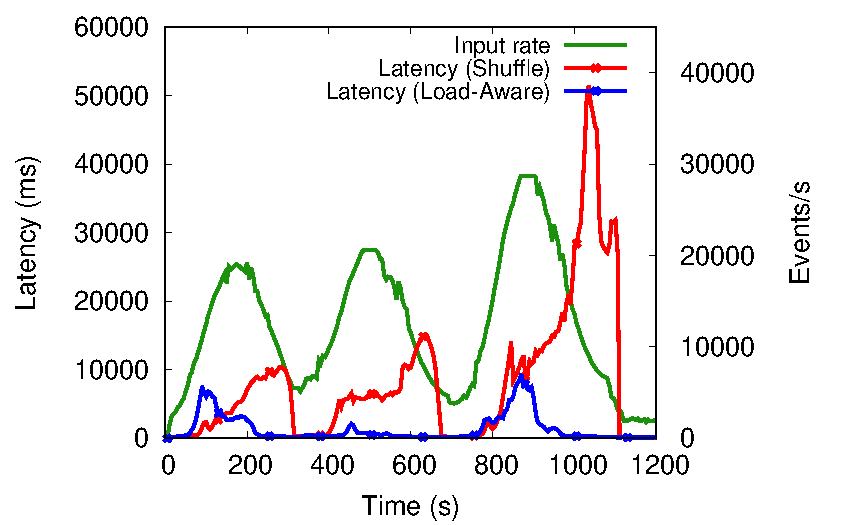
\includegraphics[width=0.75\textwidth]{figures/exp/storm/Grouping-Latency.pdf}
     \caption{Comparison of latency between \textit{Load-aware grouping} and \textit{Shuffle grouping}.}
     \label{fig:exp-grouping-latency}
\end{figure}

\subsection{Conclusion}
In this section, we have been able to evaluate the performance of our SPS, being an extension of \textit{Storm}, which has a considerable improvement to the standard version of \textit{Storm}. This is due to the limitations of the standard version.

First, we analysed the impact of the use of the replica pool, which ends up being a benefit for the SPS. This is because there is no downtime when modifying the logical resources (replicas of the operators) of the application. Secondly, we analyse the impact of a load distribution in the dispatch of events, whereby a more sophisticated strategy increases the performance of the SPS.

\section{Impact of Storm parameters}
Aiming at tuning their value, we propose in this section to discuss the impact of the two Storm parameters. The parameters are: timeout to detect the failure of an event  ($t_{out}$), and queue size ($q_{size}$). We consider that an event has failed when its processing time on all operators exceeds the end-to-end timeout, $t_{out}$. This parameter removes events that have been queued for a long time, reducing the load on an operator's replicas.

We used the \textit{Twitter Smoothed} dataset, the \textit{Twitter linear - Classification} application, \textit{Load-Aware grouping} for stream grouping strategy, and \pSPS{}, which used \textit{Basic} model for input prediction. For calculating the \textit{Saved resources} metric, we have fixed $r_{over} = 32$ (i.e., $r_i = 8$). The size of each pool of replicas ($p$) was set to 12.

\subsection{Timeout}
Table \ref{tab:exp-storm-params-timeout} shows the four scenarios, when the value of $t_{out}$ varies. 
We observe that $t_{out}$ has an impact in both  latency and loss of processed events. 
For example, a $t_{out}=1s$ improves the latency in $82.40\%$ when compared to $t_{out}=30s$ but, at the same time, there is a decrease of $9.5\%$ in the difference of processed events.  Therefore, on the one hand, if the proposed application does not require full data processing but low latency, one solution is to set the timeout to a low value for system deployment. On the other hand, if the application requires full event processing, it is recommended to use a high timeout value.

\begin{table}[!ht]
\centering
\begin{tabular}{|l|llll|}
\hline Timeout
& \begin{tabular}[c]{@{}l@{}}Saved\\ Resources\end{tabular} & \begin{tabular}[c]{@{}l@{}}Throughput\\ Degradation\end{tabular} & \begin{tabular}[c]{@{}l@{}}Diff. Proc.\\ Events\end{tabular} & \begin{tabular}[c]{@{}l@{}}Latency\\ (ms)\end{tabular} \\ \hline \hline
$t_{out}=1s$      & 0.6164   & 0.1000 & 0.9030 & 369.35 \\ \hline
$t_{out}=5s$      & 0.5875   & 0.1038 & 0.9303 & 946.69 \\ \hline
$t_{out}=10s$      & 0.5633   & 0.1056 & 0.9529 & 1298.45 \\ \hline
$t_{out}=30s$      & 0.5617   & 0.1831 & 0.9987 & 2098.91 \\ \hline
\end{tabular}
\caption{System metric values with different timeout using \textit{Twitter Smoothed} dataset.}

\label{tab:exp-storm-params-timeout}
\end{table}

\subsection{Queue size}
Table \ref{tab:exp-storm-params-queue} summarizes the four scenarios values for different sizes of the pending message queue, $q_{size}$. The greater the queue size, the higher the number of queue events, thus reducing the loss rate and increasing the number of processing events (\textit{Diff. Proc. Events}), as we can observe in the table.
On the other hand,  since many incoming events are dropped when using small queues, operators are less loaded and we observe an increase of the saved resources.  %(the number of replicas computed by Equation~\ref{eq:eq-predictive} is then smaller than the ones with big queue sizes). 
For example, with $q_{size}=100$, we observe a $19.61\%$ improvement in saved resources and a $98.57\%$ decrease of the latency compared to $q_{size}=100000$. However, the number of dropped events highly increases, inducing a decrease of $46.12\%$ in processed events.

\begin{table}[!ht]
\centering
\begin{tabular}{|l|llll|}
\hline Queue size
& \begin{tabular}[c]{@{}l@{}}Saved\\ Resources\end{tabular} & \begin{tabular}[c]{@{}l@{}}Throughput\\ Degradation\end{tabular} & \begin{tabular}[c]{@{}l@{}}Diff. Proc.\\ Events\end{tabular} & \begin{tabular}[c]{@{}l@{}}Latency\\ (ms)\end{tabular} \\ \hline \hline
$q_{size} = 100$         & 0.6719   & 0.1919 & 0.6835 & 29.91  \\ \hline
$q_{size} = 1000$        & 0.6656   & 0.1375 & 0.6922 & 311.93 \\ \hline
$q_{size} = 10000$       & 0.6602   & 0.1687 & 0.7249 & 1394.56 \\ \hline
$q_{size} = 100000$      & 0.5617   & 0.1831 & 0.9987 & 2098.91 \\ \hline
\end{tabular}
\caption{System metric values with different queue size using \textit{Twitter Smoothed} dataset.}
\label{tab:exp-storm-params-queue}
\end{table}

\subsection{Discussion}
In this section, we have observed the impact on the processing of the number of events, which can decrease depending on the chosen configuration. The timeout parameter ($t_{out}$) is inversely proportional to the latency and inversely proportional to the percentage of processed events, because as its timeout decreases, events that take a long time to process are discarded. The same happens with the queue size ($q_{size}$), so it is only recommended to use low values for both parameters if there is a very limited amount of resources.